\documentclass[]{article}

\usepackage[pdftex]{graphicx}
\usepackage[top=1in, bottom=1in, right=1.25in, left=1.25in]{geometry}
\usepackage{hyperref}

\begin{document}

	\setlength{\parindent}{0pt}
	\setlength{\parskip}{6pt}

	% Title Page
	\begin{titlepage}



		\title{\textbf{Proposed Design Report}}
		\author{BU ProPANE Team:\\Griffin Dunn\\Colin Madigan\\Phillip Stahlfeld}
		\date{November 29, 2012}
		\maketitle



		\noindent
		The purpose of this report is to present the design the BU ProPANE team will be implementing and testing in the upcoming semester. The report includes a design overview, design specifics, budget, and tentative schedule for the spring semester. The schedule will include a list of demonstrations to be completed while working towards Version 1.0 of the ProPANE system. 
		\thispagestyle{empty}
		
		
		
	\end{titlepage}
	
	
	
	
	% Begin  Real  Document
	\pagenumbering{roman}
	\tableofcontents
	\newpage
	
	\pagenumbering{arabic}
	\setcounter{page}{1}
	\thispagestyle{empty}
	
	\section{Design Overview}
		The goal of this section is to provide a high-level overview of the proposed design for the BU ProPANE system. It provides a view of the approach to the problem without diving into implementation level details. 
		
		\subsection{Concept of Operation}
			As mentioned in previous documentation concerning this project (found here: \url{http://sites.google.com/site/bupropane}), the ProPANE system will be broken down into the capture system and the analysis system. The purpose of the capture system is to collect images of a whiteboard throughout the course of a normal class. The purpose of the analysis system is to process these images for the purpose of generating key images. Figure \ref{img:concept-of-operation} shows the concept of operation for the system. There can be multiple capture systems that send images to a single analysis system for processing. 
			
			\begin{figure}[h]
				\centering
				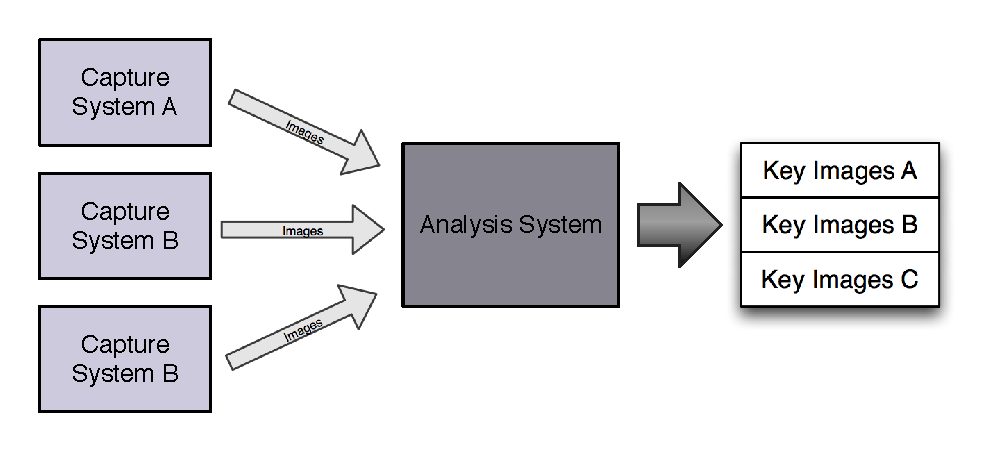
\includegraphics[scale=0.8]{images/concept-of-operation.eps}
				\caption{This figure shows the concept of operation for the overall ProPANE system. Capture systems capture images of whiteboards and send the images to the analysis system. The analysis system processes the images and generates the key images that the user desires.}		
				\label{img:concept-of-operation}
			\end{figure}
		
		\subsection{Capture System Overview}
			The capture system is a camera mounted on a tripod facing the whiteboard where information is to be captured. This setup can be seen in Figure \ref{img:setup-capture-system}. The camera will be installed with a piece of software that will take pictures periodically throughout the course of a lecture and save them to a local storage medium. These collected images can then be transferred to the analysis system for generating the desired key images. 
			
			\begin{figure}[h]
				\centering
				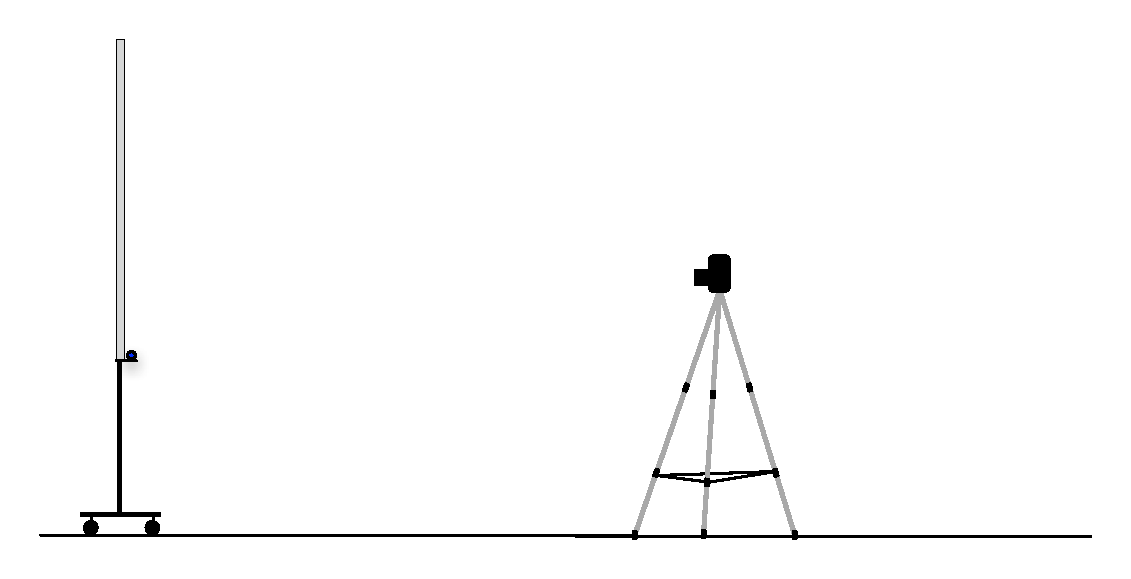
\includegraphics[scale=0.8]{images/setup-capture-system.eps}
				\caption{This figure shows the setup for the capture system with the camera on a tripod facing the whiteboard where the professor will be lecturing. Note that the capture system could be placed on a desk or table depending on the desired tripod.}		
				\label{img:setup-capture-system}
			\end{figure}
		
			
		
	\section{Capture System}
		The capture system is composed of capture device and capture stand. The BU ProPANE team has decided to use the Samsung Galaxy Camera for the capture device and the Sony VCT-R100 Tripod. 
			
			\subsection{Camera}
				The Samsung Galaxy Camera is an Android-based point-and-shoot digital camera. This device was selected for the project because it met the required criteria better than the other cameras that were examined. 
				
				\subsubsection{Camera Criteria}
					The following is a list of criteria that the camera had to meet based on the requirements documented in the technical specifications for this project:
					\begin{itemize}
						\item Programmable to allow for automatic, repetitive captures
						\item Battery capacity to allow for a full lecture of captures
						\item Portable to allow for transportation between rooms
						\item High enough resolution to discern characters within specified operating distance
					\end{itemize}
				
				\subsubsection{Camera Comparisons}
					After coming across a Microsoft Research paper documenting a solution to an extremely similar whiteboard problem, the initial idea was to use the same approach as the Microsoft team and connect a camera via USB to a computer that would signal for the camera to take a picture. Conferring with the clients resulted in this idea violating the programmable requirement for the camera because the clients desired a wireless solution. 
					
					Further research into programmable cameras resulted in the discovery of several Android-based cameras. Of the cameras on the market during the research period (beginning of October 2012), the Nikon Coolpix S800 was the forerunner since---according to user reviews---it provided the most suitable interface for programming. However, further research into the camera revealed that the battery for the camera was only capable of taking approximately 150 shots per charge. For a 52 minute class, the camera will be required to take at least 624 pictures (i.e. one picture every five seconds).
					
					Continued research yielded an advertisement for the Samsung Galaxy Camera. The Samsung Galaxy Camera has a greater programmability, larger battery (7 hours), and higher resolution than the Nikon Coolpix S800.
				
			\subsection{Sony VCT-R100 Tripod}
				After examining several different tripods, the Sony VCT-R100 seemed to be the best fit for this project. The tripod was designed to fit in a backpack so it complies with the goal of portability for the project. The only other factors that had a significant impact on the decision were weight and size. At 1.8 pounds, the tripod falls well within the 5 pound weight requirement listed in the technical specifications. When collapsed, the tripod is only 14.8 inches and designed to be carried in a backpack so again the tripod met the dimensional requirements laid out in the technical specifications. When extended, the tripod will raise the camera 39 inches above the ground, which is just above the height where the test-bed images were captured from. 
			
			\subsection{Application}
				Since the Samsung Galaxy Camera runs Android 4.1 Jelly Bean, the capture system will be based around an Android application. The Android API has an interface for cameras that let the programmer perform actions such as: taking a picture, autofocusing the camera, and saving the resulting picture as a JPEG. The following sections document the proposed design for the application.
				
				\subsubsection{Graphical Layout}
					The layout for the system was designed to separate the configuration of a capture from the capture itself. The initial screen that the user will see is Figure \ref{img:app-main-layout} where he will be able to configure how often pictures will be taken and the name of the directory where pictures will be stored (the name of the capture). Once the user clicks on the "Continue" button, he will be taken to the screen seen in Figure \ref{img:app-preview-layout} where he will be able to adjust the camera angle/focus/etc to capture the desired portions of a whiteboard. Once the ``Start Capture" button is clicked, the system will start capturing images. The ``Stop Capture" button will stop the system from capturing images and return it to the initial screen. 
					
					The first iteration of the capture system's interface was designated as a demonstration for this semester so it can be seen in Figure \ref{img:screenshot-app-preview}. Note that this is running on a Motorola Droid RAZR Maxx running Android 4.0 and has not been tested on the Samsung Galaxy Camera running Android 4.1. 
									
					\begin{figure}
						\centering
						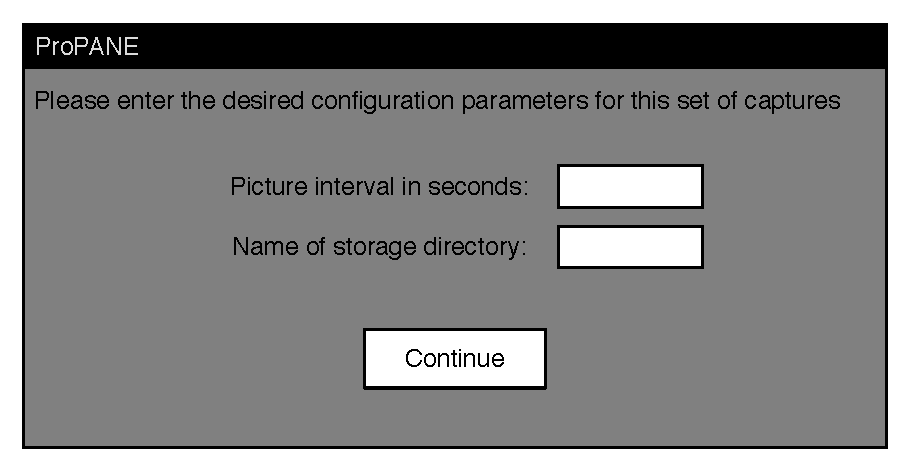
\includegraphics{images/app-main-layout-eps-converted-to.pdf}
						\caption{This figure shows the planned layout for the capture system's initial screen/Android activity.}
						\label{img:app-main-layout}
					\end{figure}
					
					\begin{figure}
						\centering
						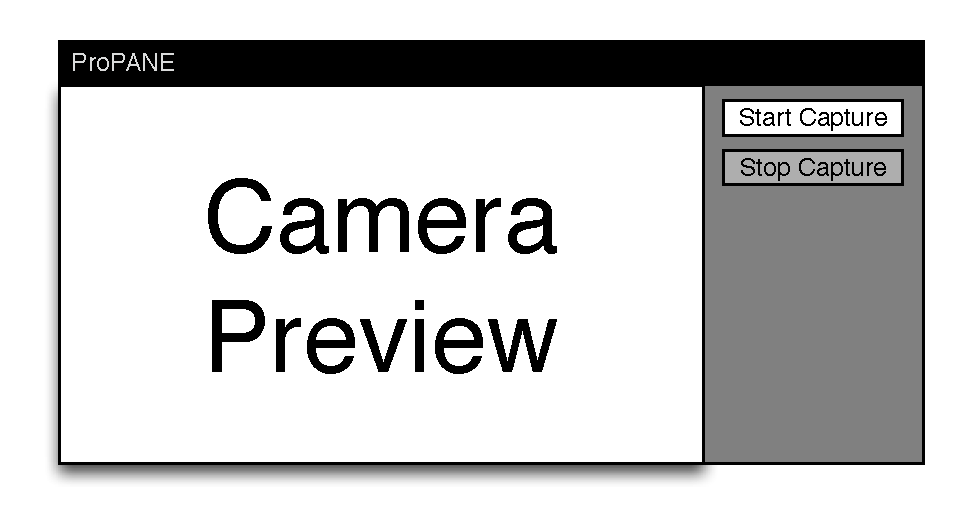
\includegraphics{images/app-preview-layout.eps}
						\caption{This figure shows the planned layout for the capture system's screen/Android activity that provides the ability to preview what part of the whiteboard will be captured by the system. Note that once the user clicks on the ``Start Capture" button, the ``End Capture" button will become enabled and the ``Start Capture" will become disabled.}
						\label{img:app-preview-layout}
					\end{figure}
					
					\begin{figure}
						\centering
						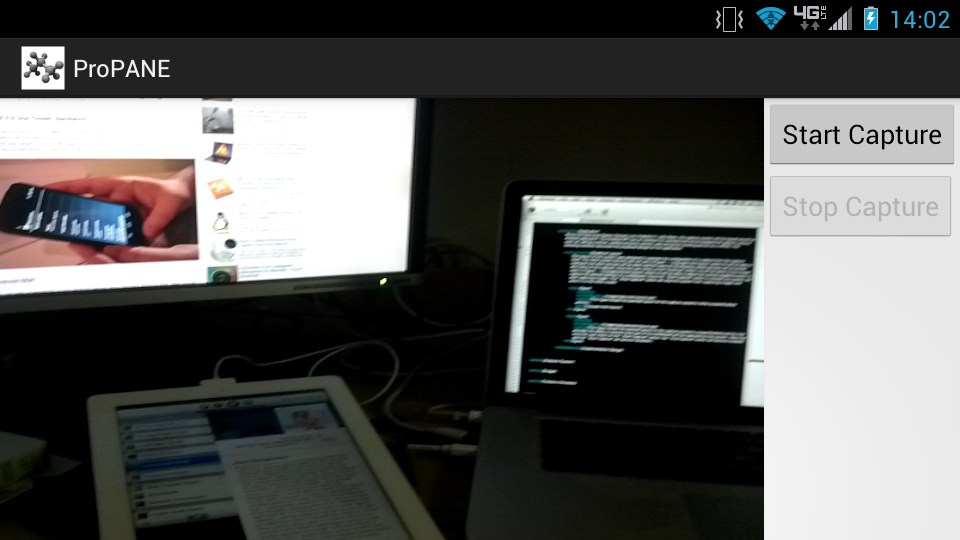
\includegraphics[scale=0.4]{images/screenshot-app-preview.png}
						\caption{This figure shows the first iteration of the app for the capture system}
						\label{img:screenshot-app-preview}
					\end{figure}
					
					
					
				\subsubsection{Class Design}
					For the full class diagram for the capture system app, see Figure \ref{img:uml-capture-system}. The main classes to focus on are MainScreen and PreviewScreen because they represent the two screen that will be shown to the user. The Preview class is just used to display what the camera is currently viewing.
					
					The MainScreen is responsible for creating the initial interface that the user sees (Figure \ref{img:app-main-layout}), collecting the necessary input from the user (picture interval, storage directory), sending that information to the PreviewScreen, and starting the PreviewScreen Activity. The design for the MainScreen will be done using the standard I/O classes provided by the Android SDK since it does not require a special component (such as a preview for the camera). Sending the input to the PreviewScreen activity will be accomplished through the use of Android Intents, which are designed to start new Activities and pass those Activities values from the creator. The ProPANE team has completed the Intents tutorial on the \url{http://developer.android.com} site demonstrating that they are capable of implementing this portion of the design. 
					
					The PreviewScreen is responsible for showing the user a preview of what to capture and creating an interface for starting/stopping the capture. When the user presses the ``Start Capture" button, the Activity will start a Service that autofocuses the camera and repeatedly takes pictures at the specified interval until the ``Stop Capture" button is pressed. The Service is needed because the capturing must still be happening when the screen goes to sleep. This is necessary to save battery power on the Samsung Galaxy Camera by putting the screen to sleep during the hour long captures. The Preview SurfaceHolder seen in the class diagram is the component that connects the PreviewScreen to the output from the camera. This feature is currently functional in the demonstration app as seen in Figure \ref{img:screenshot-app-preview}. 
					
					\begin{figure}
						\centering
						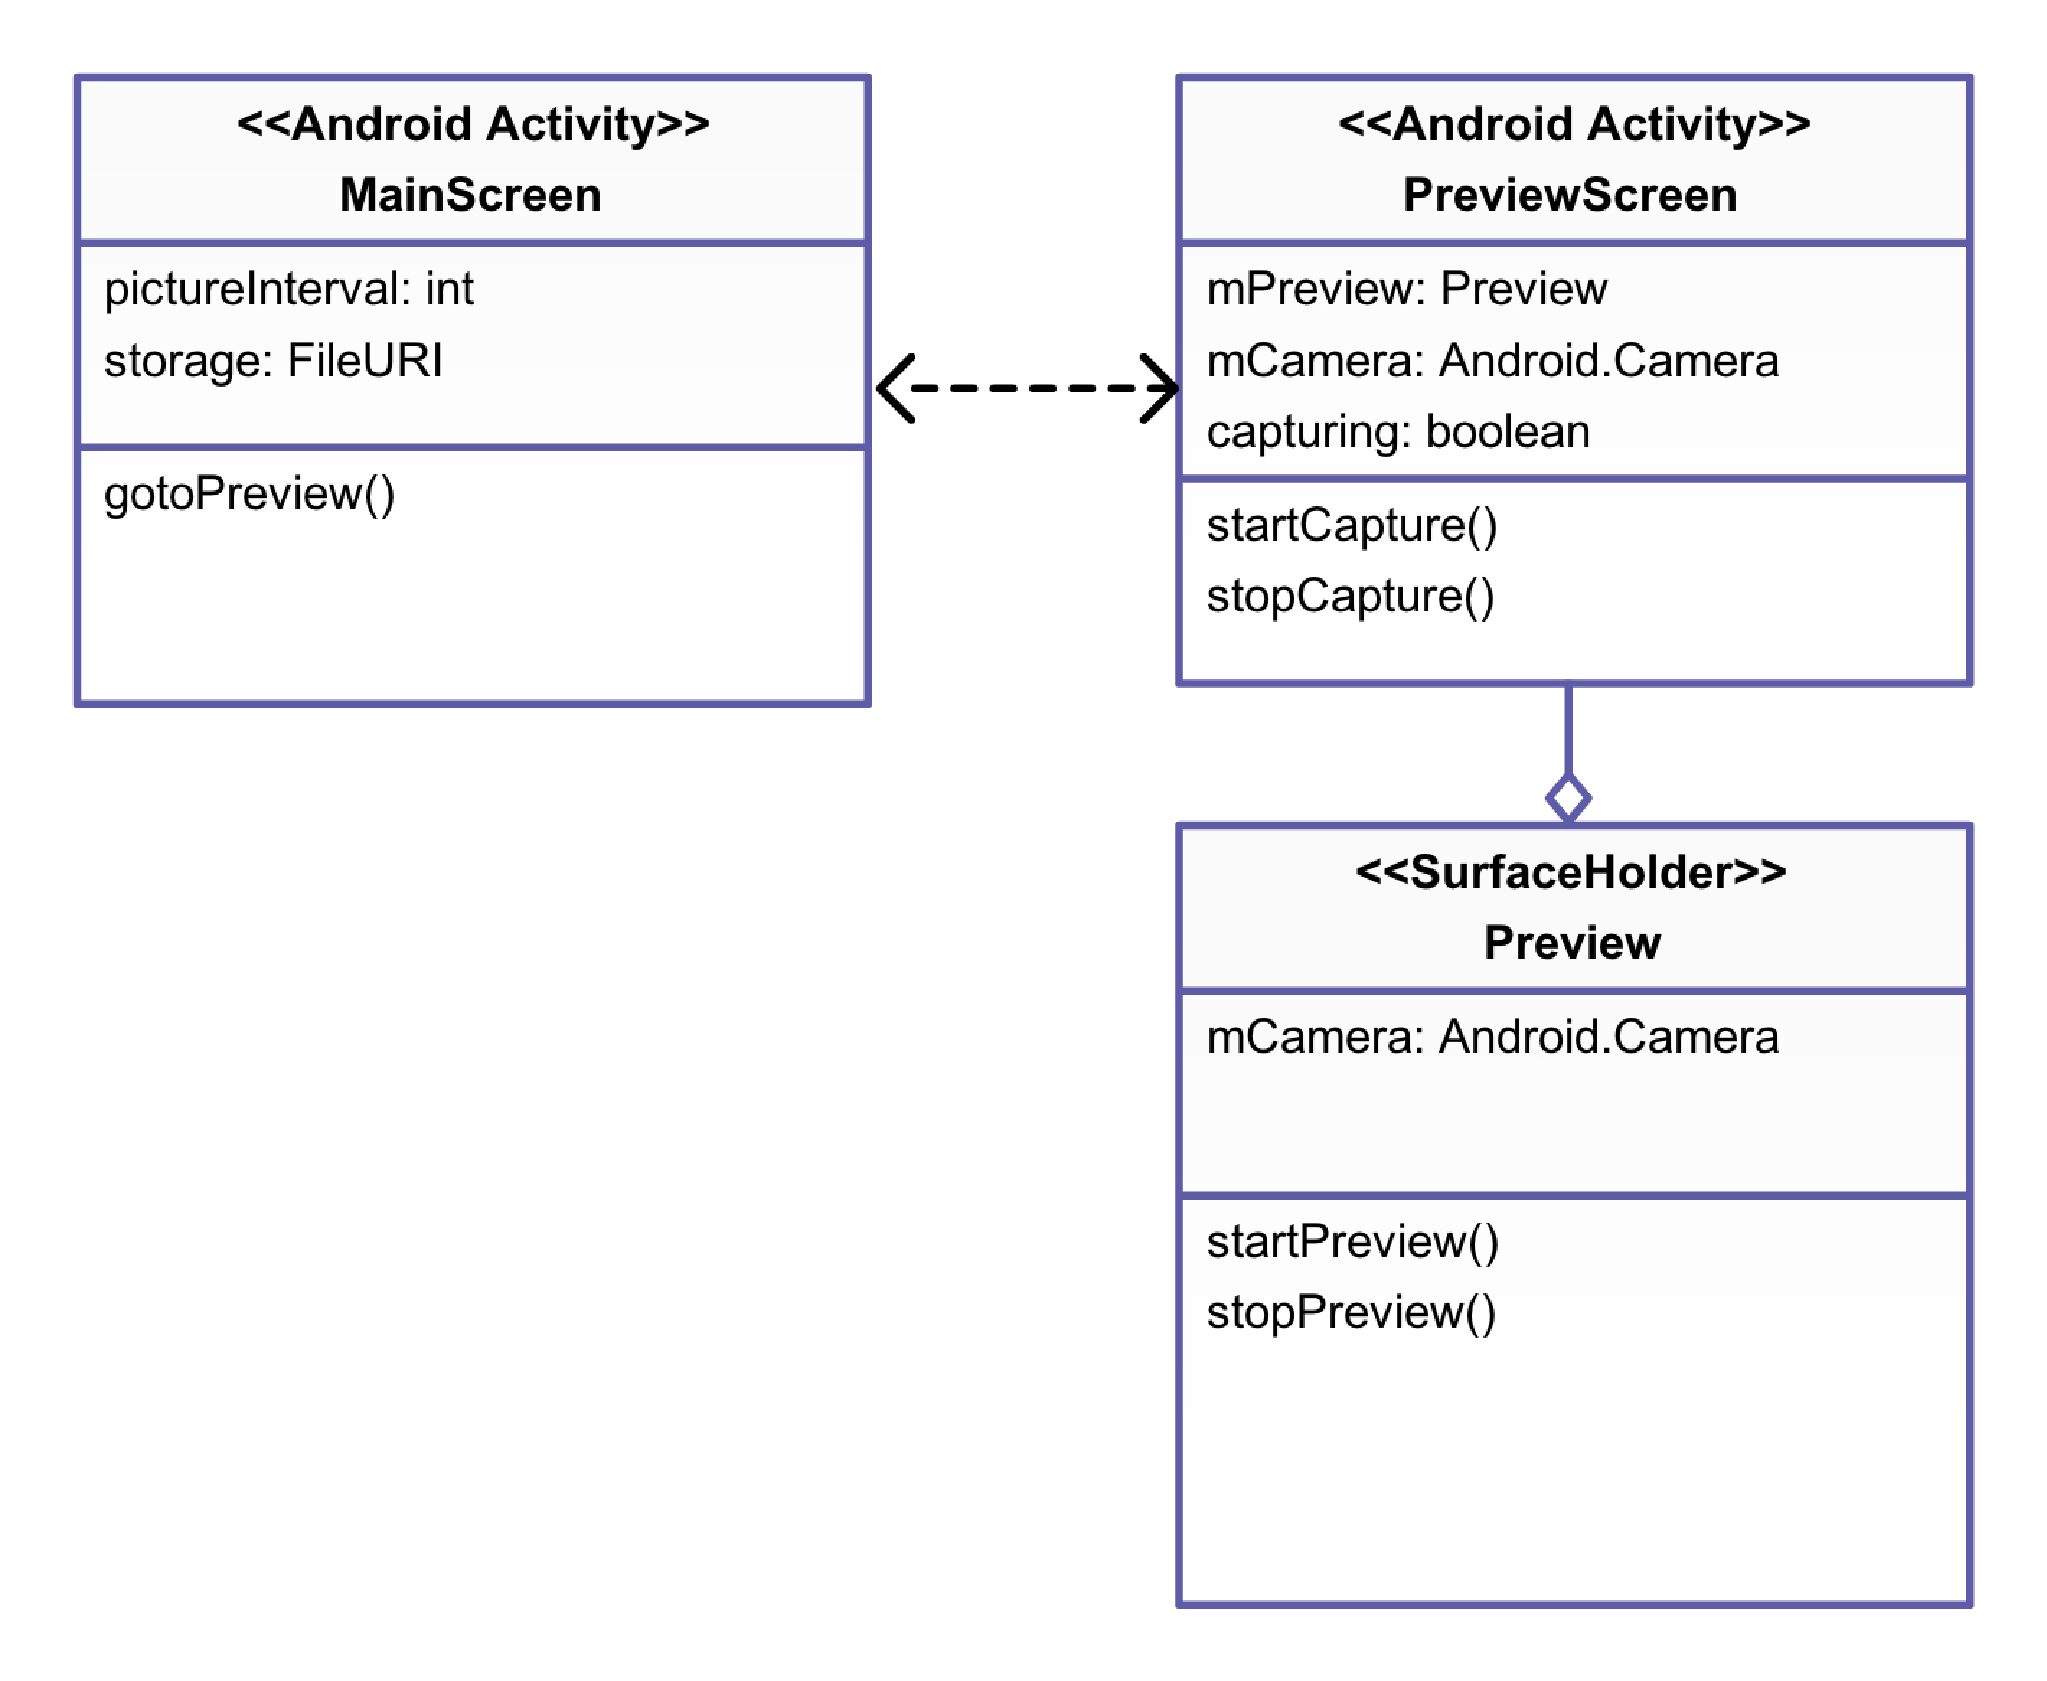
\includegraphics[scale=0.3]{images/uml-capture-system.pdf}
						\caption{This figure shows the class diagram for the Android based capture system app}
						\label{img:uml-capture-system}
					\end{figure}
	
	
	\section{Analysis System}
		The purpose of the analysis system is to process the images from the capture system. The input to the system is a collection of images from a class period and the output from the system is a smaller collection of images that represent key frames from the class period. A key frame represents a period in time just before a professor begins to erase a portion of the board. If the professor is covering a portion of the board in one of the key frames, the analysis system is responsible for stitching together previous images to remove the professor from the key frame.  
		
		\subsection{Hardware}
			The analysis system will be developed and tested on an Optiplex 475 that was provided for this project by Bucknell University. This machine has an Intel Core 2 Duo processor and 4 Gigabytes of RAM and should be more than sufficient to handle the image processing portion of this project. 
		\subsection{Software}
			After researching OpenCV, CamScanner, JMagik, and PIL (Python Imaging Library) as image processing tools, PIL was chosen as the tool for implementing the analysis system. The requirements that the tool would have to meet are as follows:
			\begin{itemize}
				\item Provide a means to stitch images
				\item Provide enough documentation to use the tool effectively
				\item Install on the Linux operating system
			\end{itemize}
			
			While OpenCV provides image stitching abilities and thousands of other tools, the package was known to cause problems when installing on Linux and the ProPANE team was not able to get the bindings for C++, Java, or Python to work correctly on the development platform. The CamScanner app for Android provided the best tools for filtering images to highlight the information written on whiteboards, but it did not provide image stitching capabilities. JMagik seemed to provide image stitching abilities and installed relatively easily, but there was essentially no documentation that showed how to use the tool effectively. Finally, PIL was included in the Python 2.7 distribution, provided a crop/paste functionality for image stitching, and plenty of documentation is available online for using it. 
			
		\subsection{Class Design}
			Given the size of this project, the best approach is to follow an object oriented design. While Python is known for being a scripting language, it contains many of the same object-oriented features as Java. To see the overall class diagram for the analysis system, see Figure \ref{img:uml-analysis-system}. The following subsections describe the classes seen in the class diagram. 
			
				\subsubsection{ImageSequence}
					This class represents a collection of images that have been taken during a single class period. This is the highest level of the system so it performs the majority of the image processing to generate key images. This is the level of the system where image stitching can take place because this class can copy cells from one image and paste them into another image. 
					
				\subsubsection{Image}
					This class represents a single image that has been taken by the capture system. This level of the system provides an organizational scheme for cells and an interface for accessing individual cells (for image stitching). 
			
				\subsubsection{Cell}
					This class represents a rectangular area on the whiteboard. The purpose of this class is to allow a single image of the whiteboard to be broken down into interchangeable pieces.
					
				\subsubsection{CellType}
					This enumeration is for the purpose of classifying cells. A board cell is just white and does not contain any foreground (i.e. the professor) or marker strokes. A stroke cell contains information that has been written on the board. A foreground cell is anything that is not part of the whiteboard.
					
			
			\begin{figure}
				\centering
				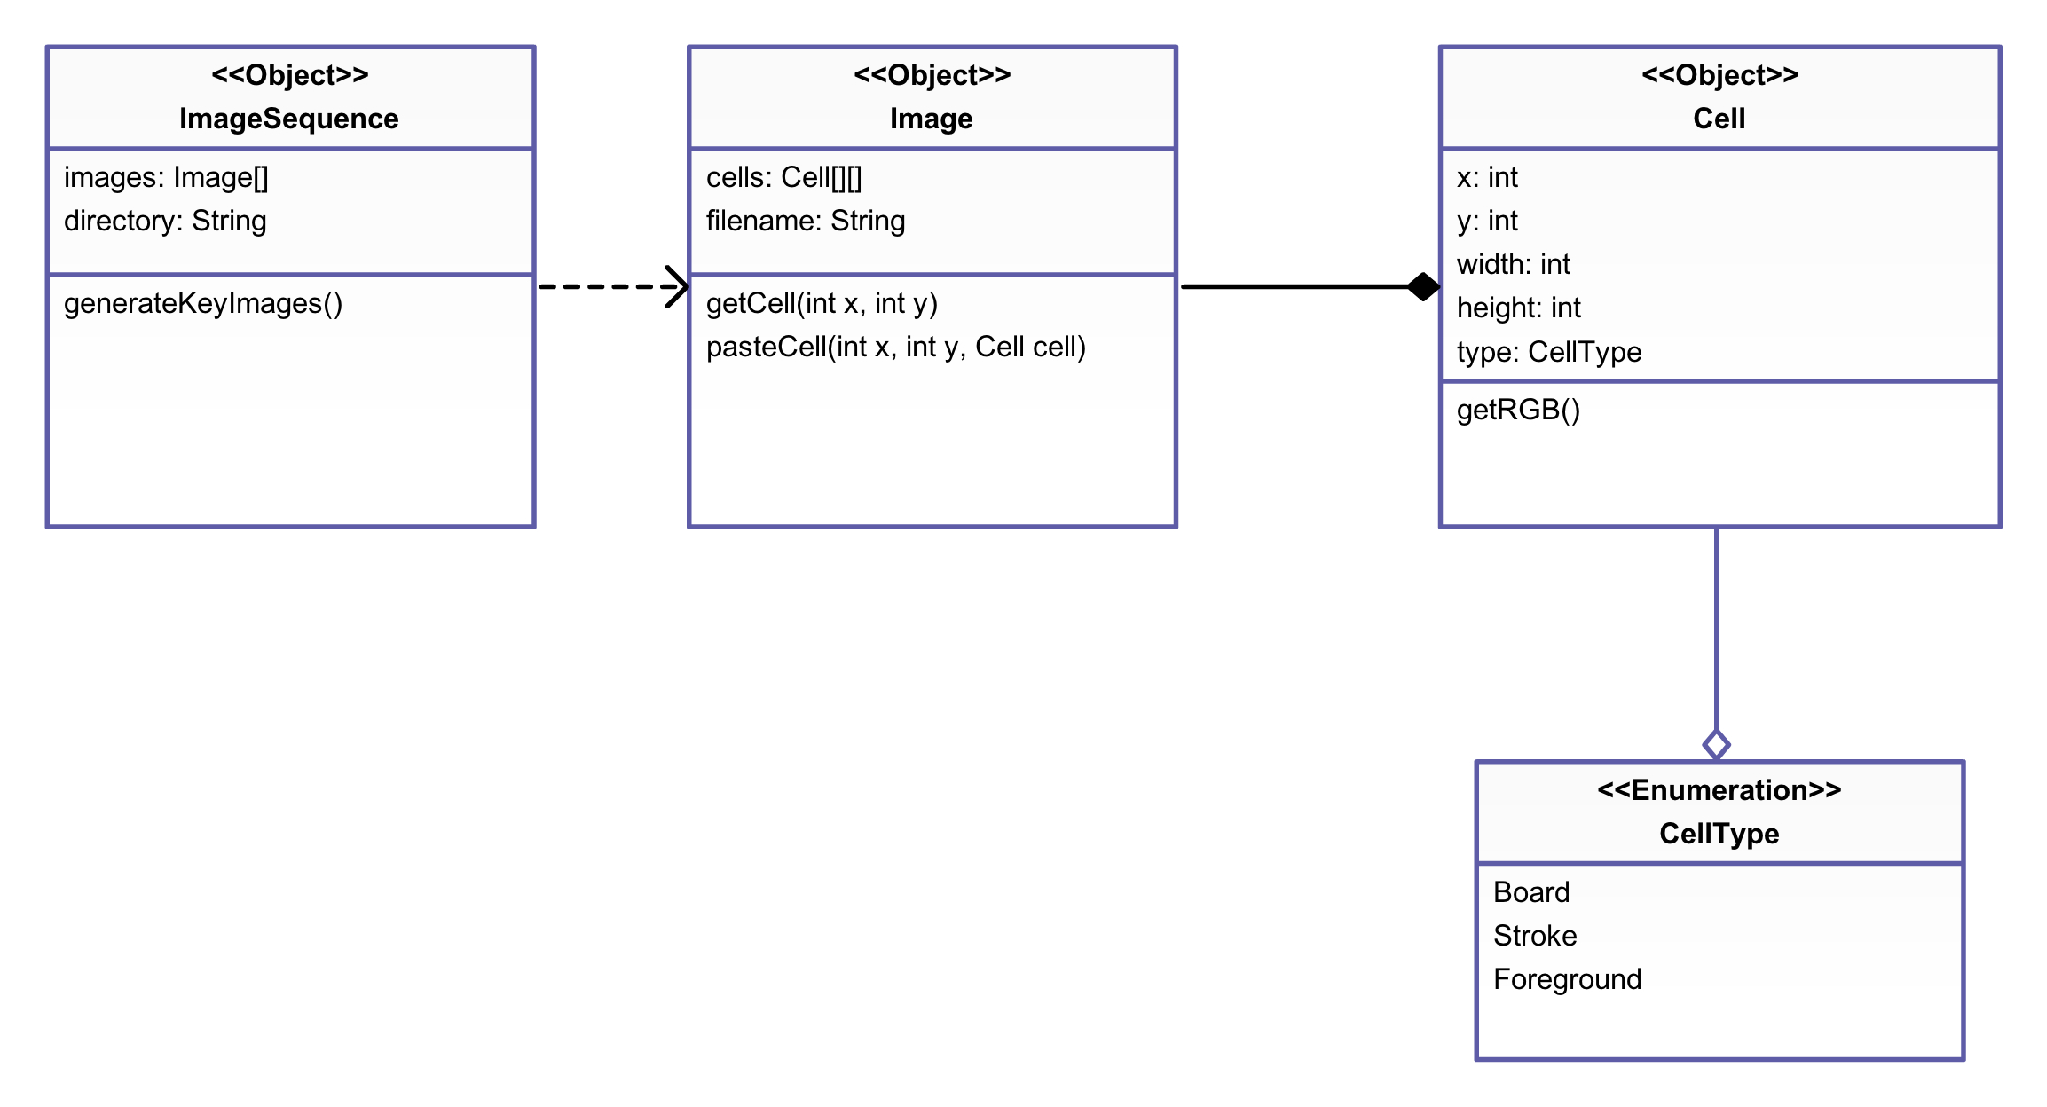
\includegraphics[scale=0.5]{images/uml-analysis-system.pdf}
				\caption{This figure shows the class diagram for the Python based analysis system}
				\label{img:uml-analysis-system}
			\end{figure}
			
		\subsection{Cell Classification}
			After an image is divided into cells, the cells must be classified as either board, stroke, or foreground cells, for the purpose of identifying when information is written on the board and when image stitching is necessary.  This is done by using the whiteboard color and standard deviation and the mean and standard deviation of the cell in question to calculate values, which are compared to set threshold values to determine the classification of the cell.  This process is detailed extensively in the background document.
			
		\subsection{Image Stitching}
			Once the amount of information on a board begins to decrease (i.e. the professor is erasing information), the system will identify the previous image as a key frame. The image stitching becomes necessary when a professor is covering part of the board during a key frame. As listed in the risk planning, image stitching presents the greatest challenge for the project. However, the object oriented design of the project has provided a straightforward solution to the problem. 
			
			Consider an ImageSequence where Image[N] has been identified as a key image and a cell at Image[N](x,y) is identified as being a foreground cell. To get the information that is being covered by the professor, the system will check to see if the cell at Image[N-1](x,y) is also foreground. The system will keep checking farther and farther back in time until it finds a cell that is not foreground. The system will then copy this cell from Image[N-n](x,y) and insert it in place of the cell at Image[N](x,y). Performing this action with any number of foreground cells will yield a view of the board without a professor covering any of the information being presented.
	
	\section{Budget}
	
		\begin{tabular}{| c | c | c | c |}
			\hline
			Item					&	Unit Cost		&	Quantity		&	Cost		\\
			\hline
			Samsung Galaxy Camera	&	\$499.99		&	1				&	\$499.99	\\
			\hline
			Sony VCT-R100			&	\$24.00			&	1				&	\$24.00 	\\
			\hline
			32 GB microSD card		&	\$22.99			&	1				&	\$22.99 	\\
			\hline
			Total					&		-			&	-				&	\$546.98+tax\\
			\hline
			
		
		\end{tabular}
	
	Our budget will only require the Galaxy Camera, a Tripod, and a microSD card. We chose the VCT-R100 because it is small, compact, and is relatively inexpensive. The microSD card was chosen because it is the largest memory card our budget can afford. See section 2 for further details on our budget reasoning.
	
	\section{Tentative Schedule}
\subsection*{Panel 4 - 2/4/13}
\begin{itemize}
\item{App on Samsung Galaxy Camera} \\

The ProPANE team will present a fully functional Android app running on the Samsung Galaxy Camera.  The app will ask the user for information on how often images should be taken and where the images will be stored.  After the user presses the ``Start Capture'' button, the app will then proceed to take images at the specified rate until the user touches the ``Stop Capture'' button.  The app will continue to take pictures even if the camera goes into sleep mode.
\item{Image stitching demo} \\

Given a set of images, the system will be able to identify and remove foreground objects, and combine images such that information originally obstructed in one or more images is visible.
\item{Key Image demo} \\

Given a set of images that have already had foreground objects removed, the system will search the set of images for key images (images that contain the maximum amount of information before a section of board is erased).  The system will identify key images and save them as independent files.
\end{itemize}

\subsection*{Panel 5 - 3/4/13}
Demonstration of a fully functional Version 1 System.  All subsections should be working together as a whole system.  This leaves room for improvement before panel 6.

\subsection*{Panel 6 - 4/15/13}
Version 1 will be 100\% complete and functional, and some features of Version 2 will be implemented.  Highest priority V2 features include image keystone correction, whiteboard normalization, automatic image cropping, and Wifi image transfer from camera to server.	
			
\end{document}